\documentclass[12pt,a4paper]{report}

% --- Paquetes de Idioma y Codificación ---
\usepackage[utf8]{inputenc}
\usepackage[T1]{fontenc}
\usepackage[english]{babel}

% --- Diseño de Página ---
\usepackage{geometry}
\geometry{top=2.5cm, bottom=2.5cm, left=3cm, right=3cm}

% --- Matemáticas y Símbolos ---
\usepackage{amsmath, amssymb, amsthm}

% --- Colores y Cajas ---
\usepackage[dvipsnames]{xcolor}
\usepackage[most]{tcolorbox}

% Caption

\usepackage{caption}

% Gráficos

\usepackage{graphicx}

% Espaciadora

\newcommand{\esp}{\vspace{0.5cm}}

% promedio

\newcommand{\prom}[1]{\left\langle #1 \right\rangle}

% Bibliografía

\usepackage[style=apa, backend=biber]{biblatex} % Estilo APA
\addbibresource{biblio.bib} % Nombre de tu archivo .bib

% Configuración de cajas personalizadas
\newtcolorbox{importante}{
	colback=red!5!white,
	colframe=red!75!black,
	title=Importante,
	fonttitle=\bfseries
}

\newtcolorbox{nota}{
	colback=blue!5!white,
	colframe=blue!75!black,
	title=Nota,
	fonttitle=\bfseries
}

% Definición de la caja de bibliografía
\newtcolorbox{bibliografia}{
	colback=gray!5!white,
	colframe=gray!75!black,
	title=Bibliografías útiles,
	fonttitle=\bfseries,
	breakable
}

% Socrative para óptica 2

\newtcolorbox{Socrative}{
	colback=orange!5!white,
	colframe=orange!75!black,
	title=Socrative,
	fonttitle=\bfseries,
	breakable
}

% Float

\usepackage{float}

% --- Hipervínculos ---
\usepackage{hyperref}
\hypersetup{
	colorlinks=true,
	linkcolor=blue,
	filecolor=magenta,      
	urlcolor=cyan,
}

% --- Datos del Documento ---
\title{Statistics Physics}
\author{Chengyu Jin}
\date{\today}

\begin{document}
	
\maketitle

\tableofcontents
\newpage

\chapter{Introduction}

\begin{figure}[H]
	\centering
	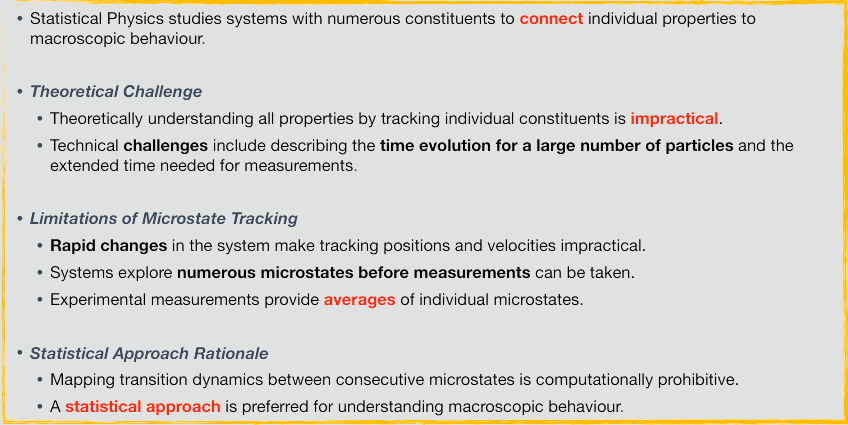
\includegraphics[width=0.7\textwidth]{IMG/statisticalapproach.png}
\end{figure}

Statistical physics is the branch of physics that studies systems composed of a large number of constituents (or \textit{degrees of freedom}). Its objective is to establish a \textbf{connection} between the essential properties of the constituents (e.g. atoms, molecules, particles) of a given system and its macroscopic or collective properties. Theoretically, one might determine the complete set of relevant properties of a system if positions and velocities of its constituents were completely known, that is if their dynamics and a model describing their mutual interactions were available. However, this approach would be immediately rejected for two main reasons: (1) describing the time evolution of, say, one mole (roughly $10^{23}$) of particles is \textbf{technically impossible} and (2) the \textbf{time needed} to observe a system and measure its properties in a given configuration is \textbf{much longer than the characteristic time} over which that system changes on a microscopic scale due to the collisions between its constituents. In other words, by the time we measure position and velocity of each atom, molecule or particle, these positions and velocities have already changed many times and the system has explored a huge number of \textit{microstates}. What one actually measures in experiments is an \textbf{average} of individual microstates. Wetherefore conclude that mapping the transition dynamics between two subsequent microstates is not only computationally prohibitive, but also uninteresting. Therefore, it makes more sense to seek a \textbf{statistical approach}. (\cite{Lecture})

\section{Microscopic and Macroscopic Perspectives}

\begin{figure}[H]
	\centering
	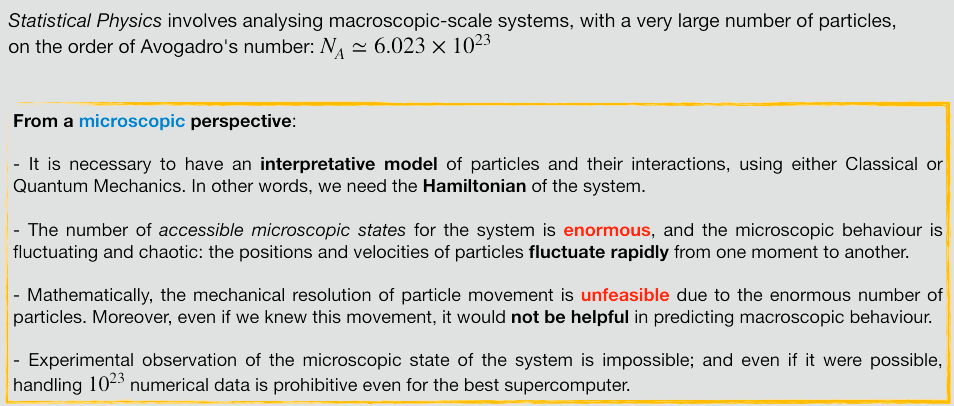
\includegraphics[width=0.7\textwidth]{IMG/microscopepersp.png}
\end{figure}

Statistical physics is a branch of Theoretical Physics that aims to provide an explanation for the macro
scopic properties of matter (mechanical, thermal, electrical, magnetic, etc.) based on the knowledge of the microscopic properties of its constituents. It employs concepts of \textbf{probability} to establish the connection between the microscopic and macroscopic universe.

\esp

To understand the behaviour of a system at the \textbf{microscopic} level, we need an interpretative model that describes the particles and their interactions. This model can be based on either \textit{Classical Mechanics} or \textit{Quantum Mechanics}, depending on the nature of the system. In either case, we rely on the system’s \textbf{Hamiltonian}, which represents its energy and governs its dynamics. One striking characteristic of the microscopic realm is the \textbf{vast} number of accessible microscopic states. The system’s particles exhibit fluctuating and chaotic behaviour, with their positions and velocities \textbf{rapidly fluctuating} over time. This dynamic nature arises from various factors, such as thermal motion, quantum effects, and the intricate interactions among particles. As already noticed above, mathematically resolving the precise motion of particles at this scale is \textbf{unfeasible} due to the \textbf{enormous} number of particles involved. Even if we had complete knowledge of their individual motions, it would \textbf{not be practical} for predicting the macroscopic behaviour of the system. This is because the macroscopic properties of the system emerge from the collective behaviour of an enormous number of particles, making it challenging to directly deduce macroscopic phenomena from microscopic dy namics. Furthermore, the experimental observation of the microscopic state of a system is \textbf{impossible in practice}. Even if it were hypothetically feasible, the sheer volume of data would be overwhelming. Handling NA number of particles is prohibitively demanding, even for the most powerful supercomputers available today. Hence, \textbf{statistical physics offers an alternative approach}. Instead of focusing on individual
particle details, it seeks to describe and understand the behaviour of macroscopic systems through statistical analysis and probability. By examining the statistical properties of ensembles of particles, statistical physics allows us to derive macroscopic laws and make predictions about observable phenomena.

\esp

\begin{figure}[H]
	\centering
	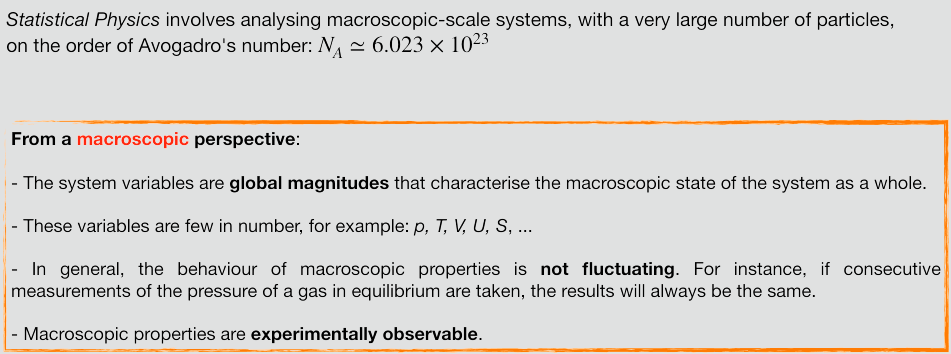
\includegraphics[width=0.7\textwidth]{IMG/macroscopepersp.png}
\end{figure}

By contrast, when we examine a system from a \textbf{macroscopic} viewpoint, we focus on \textbf{global quantities} that describe the system as a whole. These quantities provide a comprehensive understanding of the system’s macroscopic state. In this context, we typically consider only a handful of variables that capture essential aspects of the system’s behaviour. For instance, variables like pressure ($\rho$), temperature ($T$), volume ($V$), internal energy ($U$), and entropy ($S$) are commonly used to characterise and analyse macroscopic systems. Unlike the microscopic level, where particles exhibit rapid and chaotic fluctuations in their positions and velocities, macroscopic properties tend to be more stable and consistent. For example, when we repeatedly measure the pressure of a gas in equilibrium, we expect to obtain the same result each time, indicating a predictable and \textbf{non-fluctuating} macroscopic behaviour. Importantly, macroscopic properties are \textbf{directly accessible} through \textbf{experimental observations}. (\cite{Lecture})

\esp

\begin{figure}[H]
	\centering
	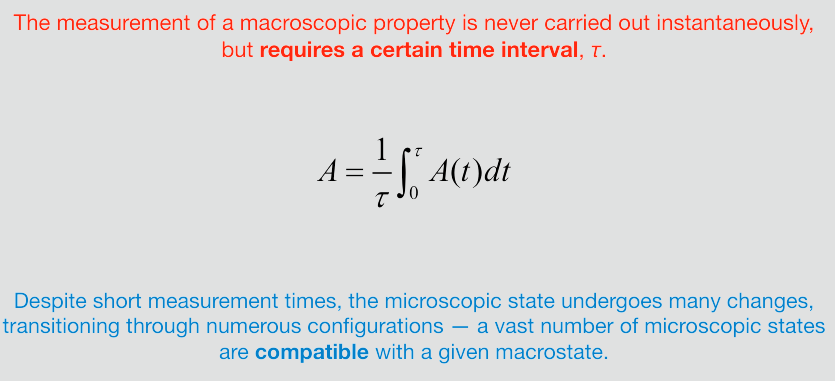
\includegraphics[width=0.7\textwidth]{IMG/instantmeasurements.png}
\end{figure}

We can measure and quantify these properties in real-world experiments, enabling us to gain insights into the behaviour and properties of macroscopic systems. It is essential to recognise that, when we perform measurements on macroscopic systems, the process takes time. Unlike the idealised concept of an instant measurement, obtaining an accurate measurement of a macroscopic property requires a finite interval of time, $\tau$. During this time interval, the system may undergo \textbf{dynamic changes or fluctuations}, which can arise from various sources, such as the inherent thermal motion of particles, external influences, or the system transitioning between different states. As a result, the measured value of the property $A$ may exhibit some degree of variability or uncertainty. It is crucial to account for this time interval when interpreting experimental results or conducting observations in statistical physics. By considering the duration of the measurement process, researchers can account for the dynamics and fluctuations that might impact the observed macroscopic properties. (\cite{Lecture})

\esp

As a general rule, even if the measurement time is very short, during that interval, the microscopic state of the system undergoes numerous changes and perturbations, transitioning through a vast number of microscopic configurations. \textbf{There exists an enormous number of microscopic states that are compatible with a given macrostate}. Regardless of the brief duration of the measurement, the microscopic constituents of the system are in constant motion and interaction. These interactions lead to continuous fluctuations and rearrangements of the particles, resulting in a multitude of possible configurations. Each
configuration represents a unique arrangement of particles with specific positions, velocities, and energy states. These fluctuations and changes occur rapidly at the microscopic level, driven by the inherent dynamics of the system. While the macroscopic properties may appear stable and predictable on average, the underlying microscopic reality is highly dynamic and constantly evolving. It is important to consider this \textbf{vast} number of microscopic states when analysing macroscopic systems using statistical physics. The ability to account for the multitude of microscopic configurations allows us to develop statistical frameworks that capture the collective behaviour of the system and derive macroscopic properties and trends. (\cite{Lecture})

\esp

\begin{figure}[H]
	\centering
	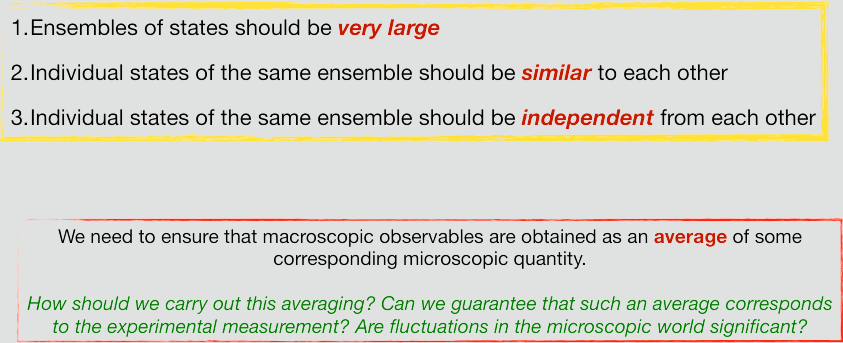
\includegraphics[width=0.7\textwidth]{IMG/statisticaltowork.png}
\end{figure}

For the application of statistics to yield good results, the following conditions are necessary:

\begin{enumerate}
	\item \textit{The ensemble of individual states must be sufficiently large}. Statistical methods rely on the principle of averaging over a large number of entities. The accuracy and reliability of statistical predictions improve as the number of individual states in the system increases.
	\item \textit{The individual states in the ensemble should share similar features}. Statistical methods assume some level of similarity or homogeneity among the individual states of the system. This assumption allows us to make generalisations and derive meaningful statistical relationships.
	\item \textit{The individuals in the ensemble should be independent}. Statistical methods assume that individual states of the system are independent of each other. This independence ensures that the statistical analysis accurately reflects the behaviour of the system as a whole.
\end{enumerate}

To obtain macroscopic observables as an average of corresponding microscopic quantities, we need to perform an appropriate averaging process. The specific method of averaging depends on the system and the properties under investigation. In statistical physics, the averaging process often involves calculating \textbf{ensemble averages} or taking \textbf{time averages} over a large number of measurements. While we aim to match the average obtained through statistical analysis with experimental measurements, it is essential to recognise the role of \textbf{fluctuations} in the microscopic world. Fluctuations occur due to the inherent probabilistic nature of microscopic phenomena. While the average behaviour can be accurately described by statistical methods, individual measurements may deviate due to these fluctuations. Statistical physics provides a framework to understand and quantify the impact of fluctuations. By examining statistical properties, such as variances and probability distributions, we can gain insights into the magnitude and significance of fluctuations and determine the range of expected deviations from the average behaviour. (\cite{Lecture})

\section{Statistical Physics and Thermodynamics}

\begin{figure}[H]
	\centering
	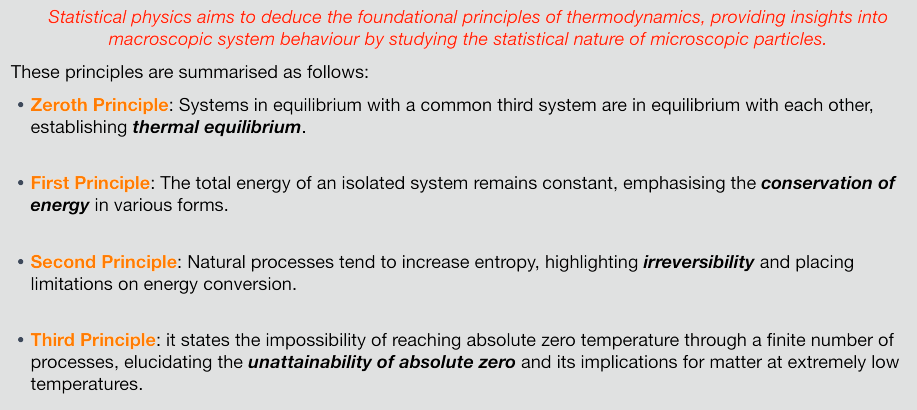
\includegraphics[width=0.7\textwidth]{IMG/thermodynamics.png}
\end{figure}

Another fundamental objective of statistical physics is to deduce the laws or principles on which thermodynamics is based. These principles form the foundation of thermodynamics and provide important insights to the behaviour of systems at the macroscopic level. Statistical physics aims to understand the statistical nature of these principles, studying the probabilistic behaviour of microscopic particles and their collective effects. They can be summarised as follows:

\begin{enumerate}
	\item \textit{Zeroth Principle}. If two bodies are in equilibrium with a third body, they are also in equilibrium with each other. The Zeroth Principle establishes the concept of thermal equilibrium, where systems that are in equilibrium with a common third system are also in equilibrium with each other. This principle allows us to define temperature and establish the basis for the measurement and comparison of thermal states.
	\item \textit{First Principle}. Although energy can take many forms, the total amount of energy remains constant. The First Principle, also known as the law of conservation of energy, states that the total energy of an isolated system remains constant. This principle is of utmost importance in understanding the
	interplay between different forms of energy, such as heat, work, and internal energy.
	\item \textit{Second Principle}. There is no cyclic device that can absorb heat from a single source and convert it entirely into work. The Second Principle, often associated with the concept of entropy, highlights the rreversibility of certain processes. It states that in any natural process, the entropy of an isolated system tends to increase, leading to a more disordered state. This principle provides valuable insights into the directionality of physical phenomena and the limitations on energy conversion.
	\item \textit{Third Principle}. The Third Principle, known as Nernst’s theorem, sets a limit on cooling processes by stating that it is impossible to reach absolute zero temperature through a finite number of processes. This principle elucidates the unattainability of absolute zero and its implications for the behaviour of matter at extremely low temperatures.
\end{enumerate}

\section{Some insight into combinations and probabilities. Microstates and macrostates}

\begin{figure}[H]
	\centering
	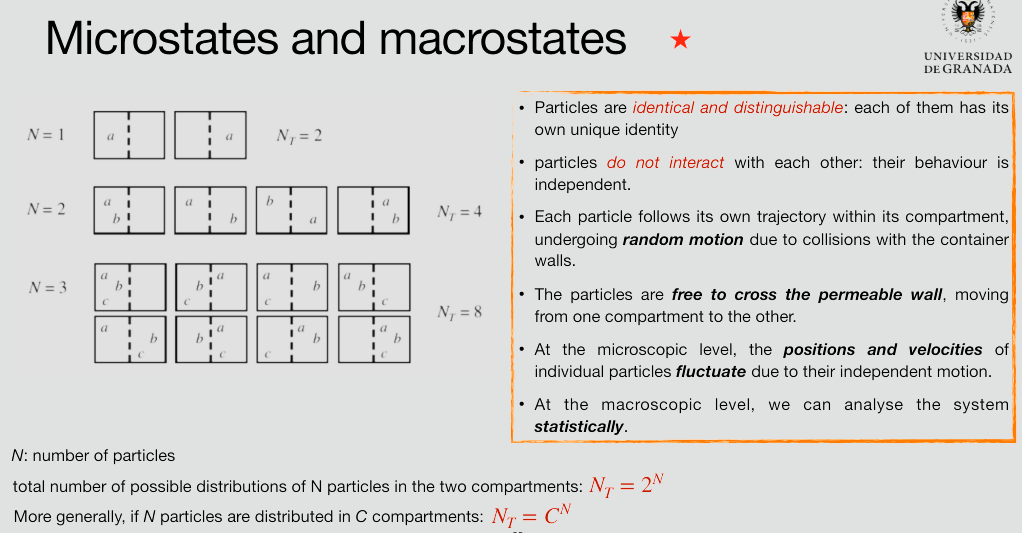
\includegraphics[width=0.7\textwidth]{IMG/microandmacro.png}
\end{figure}

In this section, we expand the ideas introduced in the above example and suggest the interested student to read Appendix A for further details on theory of probability. Here, we would like to estimate the number of microstates, $W_N(n)$, that are compatible with a given macrostate consisting of n particles in the left compartment and $N$-$n$ particles in the right compartment. Because both compartments are supposed identical, left and right are interchangeable. 

\esp

\begin{figure}[H]
	\centering
	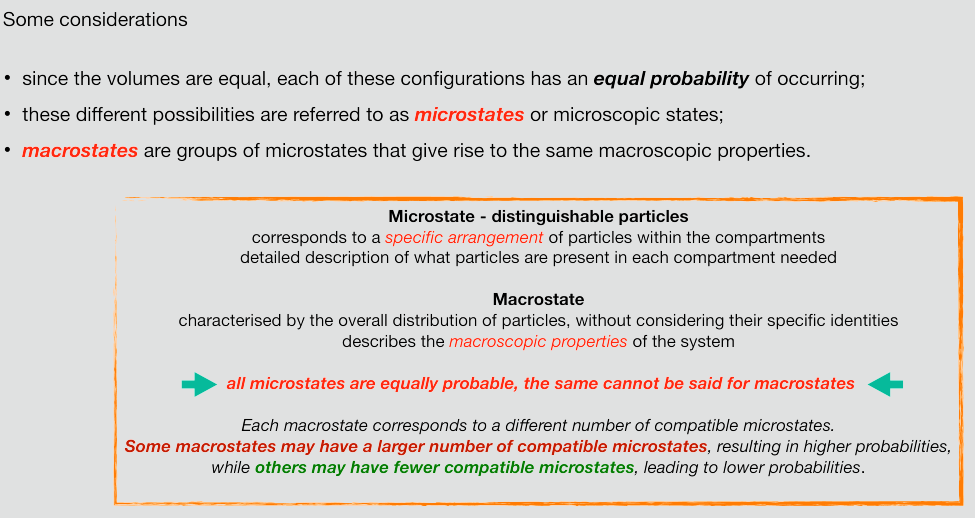
\includegraphics[width=0.7\textwidth]{IMG/considerations.png}
\end{figure}

\esp

\begin{figure}[H]
	\centering
	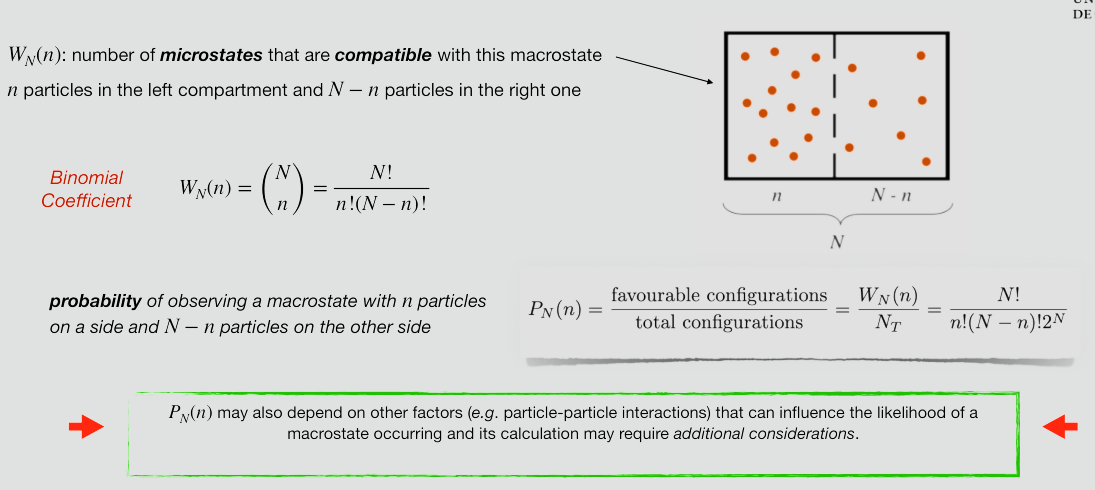
\includegraphics[width=0.7\textwidth]{IMG/combinatories.png}
\end{figure}

To this end, we need to apply combinatorial principles. More specifically, we have a total of N particles, and we want to determine the number of ways we can distribute n particles in the left compartment and $N$-$n$ particles in the right compartment. This can be visualised by arranging $N$ particles in a line and choosing $n$ of them to be in the left compartment, with the remaining $N$-$n$ particles automatically assigned to the right compartment. The number of microstates can be calculated using the binomial coefficient $\binom{N}{n}$. Mathematically, it can be expressed as

\begin{equation}
	W_N(n) = \binom{N}{n} = \frac{N!}{n!(N-n)!}
\end{equation}

The binomial coefficient accounts for all possible ways to choose n particles from the total $N$ particles, considering that the order of selection does not matter and each arrangement is considered a distinct microstate. By evaluating the binomial coefficient, we can determine the number of microstates that correspond to the given macrostate of having $n$ particles in the left compartment and $N$-$n$ particles in the right compartment. For instance, if $N = 5$ and we choose to have $n = 2$ particles in the left compartment, then we have $W_5(2)=\frac{5!}{2!3!}=10$ possible combinations of arranging our 5 particles in the two compartments. (\cite{Lecture})

\esp

Let’s take a step further. What is the probability, $P_N(n)$, of observing a macrostate with $n$ particles on a side and $N$-$n$ particles on the other side? This probability is given by the ratio of the number of microstates corresponding to that macrostate to the total number of microstates in the system. We have already mentioned that the total number of microstates or possible distributions of $N$ particles across the whole system is $N_T = 2^N$. Therefore,

\begin{equation}
	P_N(n)=\frac{favourable\ configurations}{total\ configurations} = \frac{W_N(n)}{N_T} = \frac{N!}{n!(N-n)!2^N}
	\label{eq:prob}
\end{equation}

It is important to note that in some cases, this probability may also depend on other factors such as energy considerations, constraints, or specific interactions present in the system. These additional factors can influence the likelihood of a macrostate occurring and may require additional considerations in the probability calculation.

\esp

\begin{figure}[H]
	\centering
	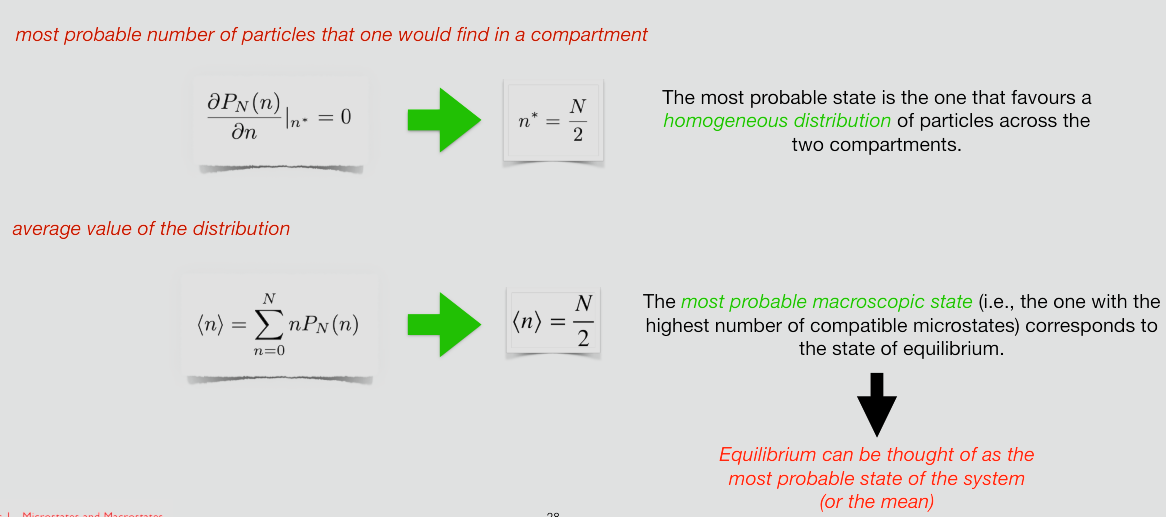
\includegraphics[width=0.7\textwidth]{IMG/mostprob.png}
\end{figure}

We first notice that the probability of finding all particles in a single compartment, that mathematically
implies that $n=N$, would result in $P_N(n=N)=1/2^N \rightarrow 0$ for large $N$. This result indicates that it is highly unlikely to find particles occupying only a single compartment. That said, it makes sense to ask the questions: what is the most probable state, $n=n^*$, and what is the probability $P_N(n^*)$ of observing thtat state? In other words, what is the most probable number of particles that one would find in a compartment? The most probable state is the one that maximises the probability $P_N(n)$:

\begin{equation}
	\frac{\partial P_N(n)}{\partial n} \Big|_{n^*} = 0
\end{equation}

\esp 

\noindent To differentiate the probability in eq (\ref{eq:prob}) with respect to $n$, we first notice that\footnote{In Statistics physics is easier use the natural logarithm}

\begin{equation}
	\frac{\partial P_N(n)}{\partial n} \Big|_{n^*} = 0 \iff \frac{\partial  \ln(P_N(n))}{\partial n} \Big|_{n^*} = 0
	\label{eq:equiv}
\end{equation}

\noindent \textbf{Demostration}. As $P_N(n) \neq 0$, then

\begin{equation*}
	\frac{\partial  \ln(P_N(n))}{\partial n} \Big|_{n^*} = \frac{1}{P_N(n)} \frac{\partial P_N(n)}{\partial n} \Big|_{n^*} = \frac{\partial P_N(n)}{\partial n} \Big|_{n^*} = 0
\end{equation*}

\noindent Differentiating eq (\ref{eq:prob}) using the equivalence showed in eq (\ref{eq:equiv}) we get

\begin{equation}
	\frac{\partial  \ln(P_N(n))}{\partial n} \Big|_{n^*} = \frac{\partial}{\partial n} \big[ \ln N! - \ln n! - \ln(N-n)! - N\ln 2 \big] \Big|_{n^*} = 0
	\label{eq:maxcondition}
\end{equation}

\noindent If $N$ is a large number, we can apply the Stirling's approximation

\begin{equation}
	\frac{\partial}{\partial n} \big[ N\ln N - N - n\ln n + n - (N-n)\ln(N-n) + (N-n) - N\ln 2 \big] \Big|_{n^*} = 0
\end{equation}

\esp

\noindent Finally, we obtain

\begin{equation}
	\ln \left(\frac{N-n^*}{n^*}\right) = 0
\end{equation}

\noindent It follows that

\begin{equation}
	\frac{N-n^*}{n^*} = 1 \implies n^* = N/2
\end{equation}

\esp

The most probable state is therefore the one that favours a homogeneous distribution of particles across the two compartments. if there were $s$ compartments, the most probable state would be $n_1 = n_2 = n_3 = \dots =
N/s$.

\esp

In light of these results, we know turn our attention to the average value of the distribution, ⟨n⟩, given by:

\begin{equation}
	\left< n \right> = \sum_{n=0}^N nP_N(n)
\end{equation}

\esp

\begin{figure}[H]
	\centering
	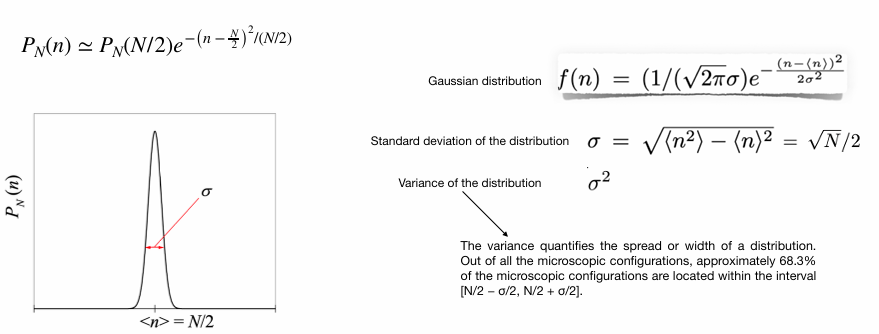
\includegraphics[width=0.7\textwidth]{IMG/gauss.png}
\end{figure}

Our aim is obtaining $\left<n\right>$. To this end, we will show that $P_N(n)$ is actually a Gaussian (normal) distribution with average $\left<n\right>$. Let’s expand the function ln $P_N(n)$ in Taylor series around $n^* = N/2$ up to the second order:

\begin{equation}
	\ln(P_N(n)) \approx \ln(P_N(n^*)) + \frac{\partial \ln(P_N(n))}{\partial n}\Big|_{n^*}(n-n^*)+\frac{1}{2}\frac{\partial^2 \ln(P_N(n))}{\partial n^2}\Big|_{n^*}(n-n^*)^2
	\label{eq:secondord}
\end{equation}

According to eq (\ref{eq:maxcondition}), the first order is zero and the second order can be simplified as 

\esp

\begin{equation}
	\frac{\partial^2 \ln(P_N(n))}{\partial n^2}\Big|_{n^*} = \frac{\partial \ln((N-n)/n)}{\partial n}\Big|_{n^*} = -\frac{1}{N-n}-\frac{1}{n}
\end{equation}

\esp

\noindent In particular at $n*= N/2$ we get

\begin{equation}
	\frac{\partial^2 \ln(P_N(n))}{\partial n^2}\Big|_{n^*} = -\frac{4}{N}
\end{equation}

\esp

\noindent Substituying these results in eq (\ref{eq:secondord}), we obtain

\begin{equation}
	\ln(P_N(n)) \approx \ln(P_N(N/2)) - \frac{2}{N}\left(n-\frac{N}{2}\right)^2 
\end{equation}

\esp

\noindent Let’s apply the exponential function to left and right hand sides:

\begin{equation}
	P_N(n) \approx P_N(N/2)e^{-\frac{2}{N}\left(n-\frac{N}{2}\right)^2} = P_N(N/2)e^{-\left(n-\frac{N}{2}\right)^2/ (N/2)}
\end{equation}

\esp

This equation highlights that is a Gaussian distribution of the type $f(n) = (1/(\sqrt{2\pi\sigma})) e^{- \frac{(n - \left< n \right>)^2}{2 \sigma^2}}$
with $n =N/2$ and $\sigma = \sqrt{N}/2$. In particular, $\sigma = \sqrt{\left< n^2 \right> - \left< n \right>^2}$ is the standard deviation of the distribution, whereas $\sigma^2$ is the variance, which quantifies the spread or width of a distribution.

\esp

\begin{figure}[H]
	\centering
	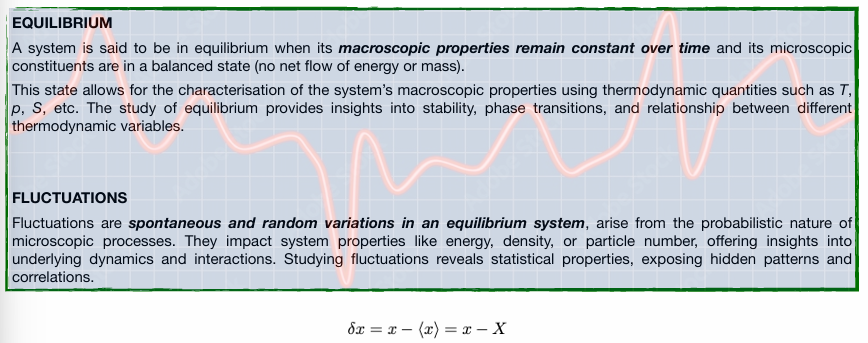
\includegraphics[width=0.7\textwidth]{IMG/eqandfluc.png}
\end{figure}

\begin{figure}[H]
	\centering
	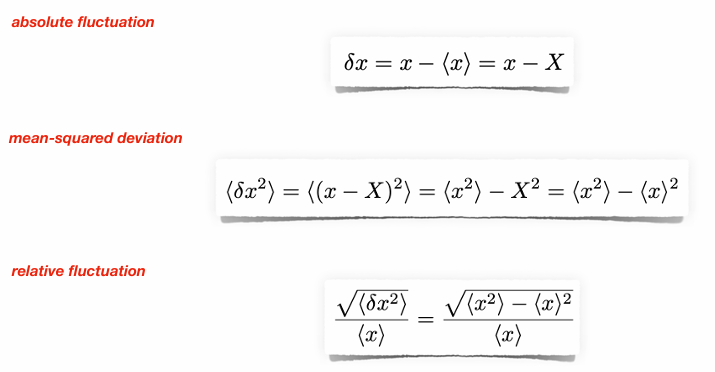
\includegraphics[width=0.7\textwidth]{IMG/typeoffluc.png}
\end{figure}

Let’s use the above example to introduce the concept of \textbf{fluctuations}. The fluctuation of a variable is a measure of how much it deviates from its average value. It is calculated by subtracting the average (also known as the mean) of the variable from its actual value. This deviation, here denoted as $\delta n$, represents the fluctuation of the variable $n$:

\begin{equation}
	\delta n = n -  \prom{n}
\end{equation}

\esp

It is important to note that fluctuations are often random in nature, meaning they can vary from one measurement to another. This can be appreciated by observing that its average over the same statistical ensemble equals zero

\begin{equation}
	\prom{n\prom{n}}=\prom{n}-\prom{\prom{n}}=\prom{n}-\prom{n}=0
\end{equation}

\esp

Consequently, the above average cannot be applied to characterise fluctuations’ intensity. In statistical physics, two commonly used measures to characterise fluctuations are the \textbf{root mean squared fluctuation} (r.m.s.) and the \textbf{relative fluctuation}:

\begin{enumerate}
	\item \textbf{Root Mean-Squared Fluctuation}. It provides a measure of the average magnitude of the fluctuations. It is calculated by taking the square root of the average of the squared deviations from the mean. Mathematically, it can be expressed as

	\begin{equation}
		\sqrt{\langle \delta n^2 \rangle} = \sqrt{\prom{(n-\prom{n})^2}} = \sqrt{\prom{(n^2-2n\prom{n}-\prom{n}^2}} = \sqrt{\prom{n^2}-\prom{n}^2}
	\end{equation}

	An advantage of the r.m.s.fluctuation is that it has the same dimensionality as the variable itself, so that the ratio between the r.m.s. fluctuation and the average value of the variable is dimensionless
	and can be employed to characterise the relative intensity of fluctuations. This ratio is defined as the \textbf{relative fluctuation}.

	\item \textbf{Relative Fluctuation}. Also known as the coefficient of variation, the relative fluctuation compares the magnitude of the fluctuation to the average value of the variable. Mathematically, it can be expressed as:
	
	\begin{equation}
		\frac{\sqrt{\prom{\delta n^2}}}{\prom{n}} = \frac{\sqrt{\prom{n^2}-\prom{n}^2}}{\prom{n}}
	\end{equation}

\end{enumerate}

\begin{figure}[H]
	\centering
	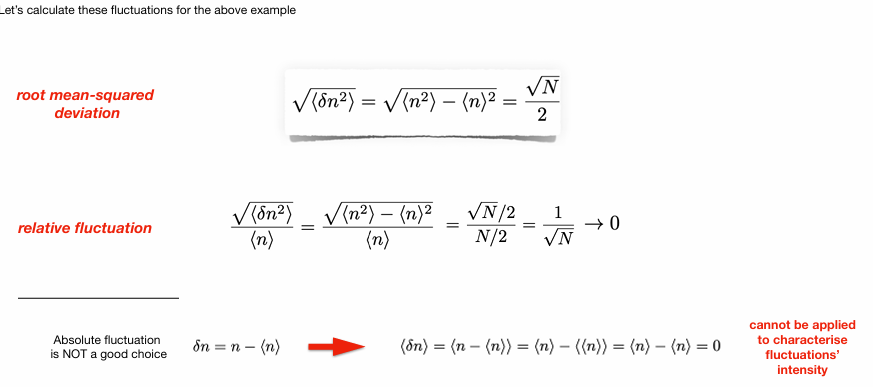
\includegraphics[width=0.7\textwidth]{IMG/example.png}
\end{figure}

Using these definitions, we can obtain the values of the root mean squared fluctuation and relative fluctuation for the system of our example:

\begin{equation}
	\sqrt{\prom{\delta n^2}} = \sqrt{\prom{n^2}-\prom{n}^2} = \sqrt{N}/2
\end{equation}

\noindent which is the standard deviation of the probability distribution $P_N(n)$ and

\begin{equation}
	\frac{\sqrt{\prom{\delta n^2}}}{\prom{n}} = \frac{\sqrt{N}/2}{N/2} = \frac{1}{\sqrt{N}}
\end{equation}

\esp

\begin{figure}[H]
	\centering
	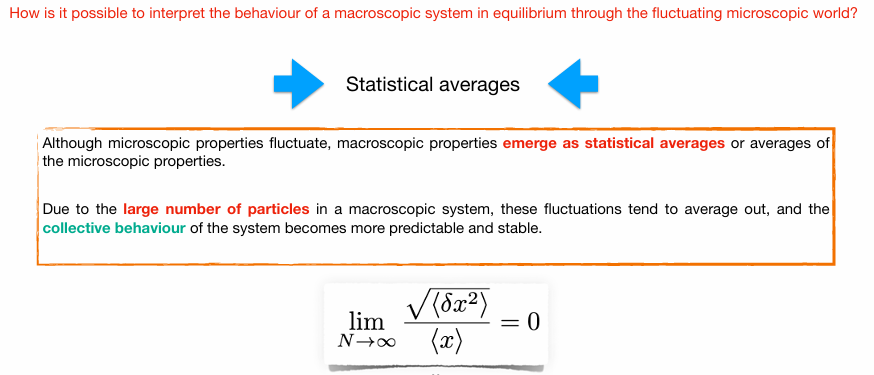
\includegraphics[width=0.7\textwidth]{IMG/statave.png}
\end{figure}

\begin{figure}[H]
	\centering
	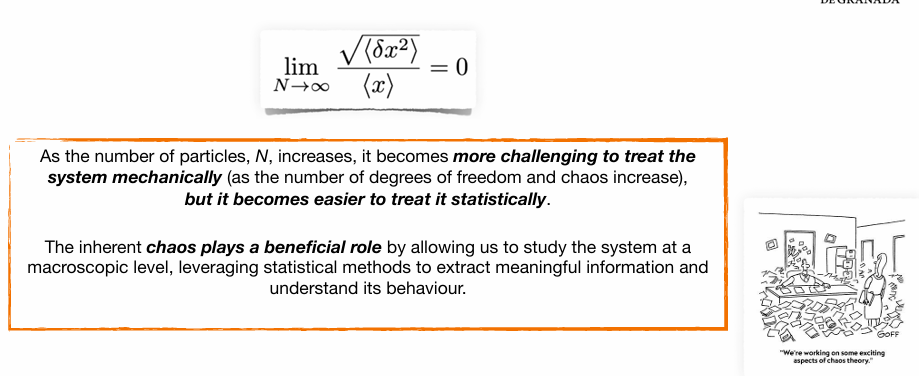
\includegraphics[width=0.7\textwidth]{IMG/vastN.png}
\end{figure}	

In a macroscopic sample, where the number of particles is on the order of Avogadro’s number, the fluctuations are on the order of $10^{-11}$ and therefore \textbf{negligible}. As the width of the distribution tends to zero, the maximum value and the mean always coincide in macroscopic systems. The probability of a macrostate that deviates from the mean value is practically zero, even for macrostates very close to the mean. When
we measure the macrostate of a system in equilibrium, the value we will always observe is the mean value. Macroscopically speaking, the system behaves as if it is always in the state $n = N/2$. The same conclusions can be applied to any other macroscopic property $A \equiv \prom{a}$ that has a corresponding microscopic counterpart associated with the particles:

\begin{equation}
	\frac{\sqrt{\prom{n^2}-A^2}}{A} \propto \frac{1}{\sqrt{N}} \rightarrow 0
\end{equation}

\esp

\begin{figure}[H]
	\centering
	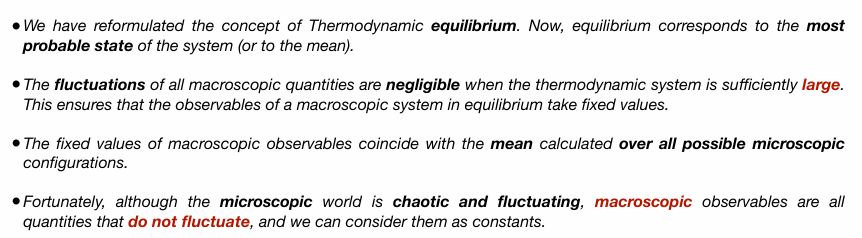
\includegraphics[width=0.7\textwidth]{IMG/conclusions.png}
\end{figure}

In this chapter, we have discussed the main goals of Statistical Physics. We have also discussed the concept of Thermodynamic Equilibrium. Equilibrium corresponds to the most probable state of the system (or the mean). The fluctuations in all macroscopic quantities are negligible when the thermodynamic system is large enough. This
guarantees that the observables of a macroscopic system in equilibrium take fixed values. The fixed values
of macroscopic observables coincide with the average over all possible microscopic configurations. \textbf{Fortunately, although the microscopic world is chaotic and fluctuating, the macroscopic observables are quantities that do not fluctuate, and we can consider them as constants}. This property allows us to treat macroscopic observables as stable and predictable quantities, even in the presence of microscopic fluctuations. It is the collective behaviour of a large number of microscopic constituents that gives rise to the stability and predictability of macroscopic systems in equilibrium. By studying the statistical properties
and averaging over all possible microscopic configurations, we can effectively describe and understand the
macroscopic behaviour of systems in equilibrium. This approach provides a powerful framework for analysing
and predicting the properties of complex systems, bridging the gap between the microscopic and macroscopic
scales of the physical world.

\printbibliography[title={Bibliografía}]
\end{document}